% !TEX program = xelatex
% =============================================================================
% Pixel Round — Технологическая карта урока (ru-RU)
% Адаптировано для 11 класса средней общеобразовательной школы России (ФГОС СОО)
% Графическая идентичность по docs_math/Pixel_Round_Math_ru-RU.pdf
% Компиляция: xelatex Plano_de_Aula_ru-RU.tex   (два прохода для содержания)
% =============================================================================
\documentclass[12pt,a4paper]{scrartcl}

% ---------- Язык и шрифты ----------------------------------------------------
\usepackage{fontspec}
\usepackage{polyglossia}
\setdefaultlanguage{russian}
\PolyglossiaSetup{russian}{indentfirst=false}
\setmainfont{Latin Modern Roman}[Scale=1.08]
\setsansfont{Latin Modern Sans}[Scale=1.08]
\setmonofont{Latin Modern Mono}[Scale=1.00]
\usepackage{unicode-math}
\setmathfont{Latin Modern Math}[Scale=1.08]

% ---------- Пакеты -----------------------------------------------------------
\usepackage{amsmath}
\usepackage{mathtools}

\usepackage[a4paper,top=2.8cm,bottom=2.8cm,left=2.6cm,right=2.6cm,
            headheight=16pt]{geometry}
\usepackage{microtype}
\usepackage{xcolor}
\usepackage{booktabs}
\usepackage{array}
\usepackage{tabularx}
\usepackage{enumitem}
\usepackage{titlesec}
\usepackage{fancyhdr}
\usepackage{graphicx}
\usepackage{csquotes}
\usepackage{tcolorbox}
\tcbuselibrary{skins,breakable}
\usepackage{needspace}                   % evita orfas em caixas didaticas
\usepackage{caption}
\usepackage{subcaption}
\usepackage{float}                       % [H] = "exatamente aqui, sem float"

\raggedbottom                            % paginas terminam onde o texto termina
\usepackage[colorlinks=true,
            linkcolor=linkc,
            urlcolor=linkc,
            citecolor=linkc,
            bookmarks=true,bookmarksopen=true,
            pdftitle={Pixel Round — Технологическая карта урока (ru-RU)},
            pdfauthor={Vinícius Rodrigues de Souza}]{hyperref}

% ---------- Цветовая палитра -------------------------------------------------
\definecolor{accent}{HTML}{CC2020}
\definecolor{ink}{HTML}{1F1F23}
\definecolor{muted}{HTML}{4E4E58}
\definecolor{bg}{HTML}{FBF6E9}
\definecolor{rule}{HTML}{D8D1BC}
\definecolor{linkc}{HTML}{8A0F0F}             % links: tom mais escuro do accent

\color{ink}

% Penalidades altas contra orfas / viuvas globalmente
\widowpenalty=10000
\clubpenalty=10000

% ---------- Стиль заголовков -------------------------------------------------
\titleformat{\section}
  {\sffamily\Large\bfseries\color{accent}}{\thesection.}{0.6em}{}
\titleformat{\subsection}
  {\sffamily\large\bfseries\color{accent!85!ink}}{\thesubsection}{0.6em}{}
\titleformat{\subsubsection}
  {\sffamily\normalsize\bfseries\color{muted}}{\thesubsubsection}{0.5em}{}
\titlespacing*{\section}{0pt}{1.2\baselineskip}{0.6\baselineskip}
\titlespacing*{\subsection}{0pt}{0.8\baselineskip}{0.3\baselineskip}
\titlespacing*{\subsubsection}{0pt}{0.6\baselineskip}{0.2\baselineskip}

% ---------- Колонтитулы ------------------------------------------------------
\pagestyle{fancy}
\fancyhf{}
\fancyhead[L]{\small\sffamily\bfseries\color{accent}PIXEL ROUND}
\fancyhead[R]{\small\sffamily\color{muted}Технологическая карта --- 11 класс}
\fancyfoot[L]{\small\sffamily\color{muted}Pixel Round --- материал для учителя}
\fancyfoot[R]{\small\sffamily\color{muted}Страница \thepage}
\renewcommand{\headrulewidth}{0.4pt}
\renewcommand{\footrulewidth}{0.4pt}
\renewcommand{\headrule}{{\color{rule}\hrule height \headrulewidth}}
\renewcommand{\footrule}{{\color{rule}\vskip-\footrulewidth\hrule height \footrulewidth\vskip-\footrulewidth}}

% ---------- Дидактические блоки ----------------------------------------------
\newtcolorbox{formula}{
  colback=bg, colframe=rule, boxrule=0.4pt, arc=2pt,
  left=10pt,right=10pt,top=8pt,bottom=8pt,
  before skip=8pt, after skip=8pt,
  fontupper=\color{accent}, breakable,
  before={\par\needspace{4\baselineskip}}
}

\newtcolorbox{zadanie}[1][Задание]{
  enhanced, breakable,
  colback=bg, colframe=accent, boxrule=0.6pt, arc=4pt,
  left=12pt,right=12pt,top=10pt,bottom=10pt,
  before skip=12pt, after skip=12pt,
  before={\par\needspace{14\baselineskip}},
  attach boxed title to top left={xshift=10pt,yshift=-8pt},
  boxed title style={colback=accent,colframe=accent,boxrule=0pt,arc=2pt},
  coltitle=white, fonttitle=\sffamily\bfseries\small,
  title=#1
}

\newtcolorbox{primechanie}[1][Методический комментарий]{
  enhanced, breakable,
  colback=bg!50!white, colframe=rule, boxrule=0.4pt, arc=2pt,
  left=10pt,right=10pt,top=8pt,bottom=8pt,
  before skip=8pt, after skip=8pt,
  before={\par\needspace{6\baselineskip}},
  attach boxed title to top left={xshift=10pt,yshift=-7pt},
  boxed title style={colback=muted,colframe=muted,boxrule=0pt,arc=2pt},
  coltitle=white, fonttitle=\sffamily\bfseries\footnotesize,
  title=#1
}

\newtcolorbox{rezultat}[1][ФГОС СОО]{
  enhanced, breakable,
  colback=bg!70!white, colframe=accent!60!ink, boxrule=0.4pt, arc=2pt,
  left=10pt,right=10pt,top=6pt,bottom=6pt,
  before skip=6pt, after skip=6pt,
  before={\par\needspace{4\baselineskip}},
  attach boxed title to top left={xshift=10pt,yshift=-6pt},
  boxed title style={colback=accent!60!ink,colframe=accent!60!ink,boxrule=0pt,arc=2pt},
  coltitle=white, fonttitle=\sffamily\bfseries\footnotesize,
  title=#1
}

\setlength{\parskip}{0.75em}
\setlength{\parindent}{0pt}
\linespread{1.10}

\newcommand{\code}[1]{\texttt{\small #1}}
\newcommand{\acc}[1]{\textcolor{accent}{\textbf{#1}}}
\newcommand{\vrema}[1]{\textnormal{\footnotesize\color{bg!90!white}\textsf{#1}}}

% Configuracao de legendas
\captionsetup{font=small, labelfont={bf,color=accent}, textfont={color=muted}, justification=centering}
\captionsetup[sub]{font=footnotesize, labelfont={bf,color=accent!75!ink}, textfont={color=muted}}

% Espacamento das figuras
\setlength{\textfloatsep}{14pt plus 2pt minus 2pt}
\setlength{\floatsep}{14pt plus 2pt minus 2pt}
\setlength{\intextsep}{14pt plus 2pt minus 2pt}

\graphicspath{{img/}}

\begin{document}

% =============================================================================
% ТИТУЛЬНЫЙ ЛИСТ
% =============================================================================
\begin{titlepage}
  \centering
  \vspace*{3.2cm}
  {\sffamily\bfseries\fontsize{56}{60}\selectfont \color{accent} Pixel Round\par}
  \vspace{0.7cm}
  {\sffamily\LARGE\color{muted} Технологическая карта урока\par}
  \vspace{0.25cm}
  {\sffamily\Large\color{muted} 11 класс --- среднее общее образование\par}
  \vspace{1.4cm}
  {\color{rule}\rule{0.6\textwidth}{0.6pt}\par}
  \vspace{0.9cm}
  \begin{minipage}{0.84\textwidth}
    \centering\color{ink}\large
    Серия из четырёх уроков, представляющая программное
    обеспечение \emph{Pixel Round} учащимся 11 классов средней
    общеобразовательной школы Российской Федерации. Объединяет
    аналитическую геометрию, алгоритмическое мышление и
    эстетическое творчество вокруг единой проблемы: как
    представить непрерывную кривую на конечной сетке пикселей.
  \end{minipage}
  \vspace{0.9cm}\\
    \vspace{1.4cm}
  \begin{minipage}{0.78\textwidth}
    \centering
    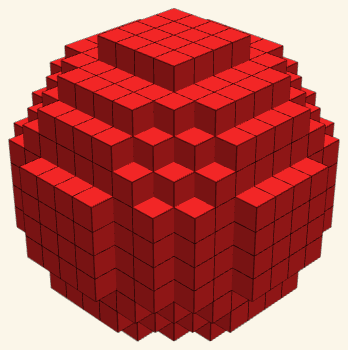
\includegraphics[width=0.55\linewidth]{fig07_3d_sphere_d12.png}\\[0.6em]
    {\sffamily\footnotesize\color{muted}Воксельная сфера диаметром 12, созданная Pixel Round.}
  \end{minipage}
  \vspace{1.0cm}\\
  {\color{rule}\rule{0.6\textwidth}{0.6pt}\par}
  \vspace{1.0cm}
{\color{rule}\rule{0.6\textwidth}{0.6pt}\par}
  \vspace{1.8cm}
  \begin{minipage}{0.82\textwidth}
    \centering\sffamily\small\color{muted}
    \textbf{Межпредметные связи:} Математика $\cdot$ Информатика $\cdot$ Изобразительное искусство $\cdot$ Физика \\[0.4em]
    \textbf{Нормативная основа:} ФГОС СОО (Приказ Минпросвещения России от 12.08.2022 № 732) $\cdot$ Примерная рабочая программа по математике
  \end{minipage}
\end{titlepage}

% =============================================================================
% СОДЕРЖАНИЕ
% =============================================================================
\renewcommand{\contentsname}{\color{accent}Содержание}
\tableofcontents
\thispagestyle{fancy}
\newpage

% =============================================================================
\section{Общие сведения}

\begin{center}
\begin{tabular}{@{}p{0.32\textwidth}p{0.62\textwidth}@{}}
\toprule
\textbf{Предмет} & Математика (профильный уровень); адаптируется для базового уровня и для предмета \emph{Информатика}. \\
\addlinespace[2pt]
\textbf{Класс} & 11. Адаптируется к 10 классу и к старшим группам учреждений СПО. \\
\addlinespace[2pt]
\textbf{Тип уроков} & Уроки открытия нового знания (1, 3), урок общеметодологической направленности (2), урок развивающего контроля (4). \\
\addlinespace[2pt]
\textbf{Время} & 4 урока по 45 минут (180 мин аудиторной работы). Спаренный вариант (две пары по 90 мин) описан в §\ref{sec:diff}. \\
\addlinespace[2pt]
\textbf{Основной ресурс} & Pixel Round --- бесплатное веб-приложение, не требует регистрации и сервера, работает в офлайн-режиме (PWA). Соответствует требованиям защиты персональных данных. \\
\addlinespace[2pt]
\textbf{Соответствие ФГОС} & Предметные результаты блока \emph{Геометрия} и \emph{Алгебра и начала математического анализа}; метапредметные результаты УУД познавательного и регулятивного характера. \\
\addlinespace[2pt]
\textbf{Межпредметные связи} & Информатика (алгоритмика, программирование на Python); ИЗО (цифровая графика); Физика (волновые процессы, акустика). \\
\addlinespace[2pt]
\textbf{Опорные знания учащихся} & Координатная плоскость и пространство; уравнение окружности; объёмы тел вращения; понятие функции; пропорция и проценты. \\
\addlinespace[2pt]
\textbf{Подготовка учителя} & 15 минут самостоятельного изучения интерфейса Pixel Round; чтение технического сопровождения \texttt{docs\_math/Pixel\_Round\_Math\_ru-RU.pdf}. \\
\bottomrule
\end{tabular}
\end{center}

\begin{primechanie}[Особенности российской школьной среды]
Серия уроков спроектирована с учётом реального положения дел в школах различных регионов России: значительная неоднородность материальной базы (от полностью укомплектованных школ Москвы и Санкт-Петербурга до сельских школ Сибири и Дальнего Востока), широкое распространение интерактивных досок и Электронного журнала, обязательная подготовка к ЕГЭ. Pixel Round работает на любом устройстве с современным браузером, не требует учётной записи и не передаёт данные на внешний сервер. \emph{Полностью автономный} вариант (без использования компьютеров) описан в Приложении~\ref{ap:adapt}.
\end{primechanie}

% =============================================================================
\section{Методологическое обоснование}

Пиксельное искусство и воксельная графика составляют значительную часть визуального опыта современного российского подростка --- от Minecraft и Stardew Valley до игр отечественной разработки (\emph{4A Games}, \emph{Mundfish}). Превращение этой повседневной эстетики в \acc{предмет математического исследования} преобразует знакомый зрительный материал в подлинную математическую проблему: как описать средствами компьютера, обладающего лишь квадратными ячейками, кривую, аналитически определённую над $\mathbb{R}$?

Серия уроков опирается на три педагогические традиции, особенно сильные в отечественной школьной математике:

\begin{itemize}[leftmargin=1.3em,itemsep=0.15em,topsep=0.3em]
  \item \acc{Системно-деятельностный подход}, лежащий в основе ФГОС. Учебная деятельность строится как последовательность действий по присвоению знаний, а не как пассивное усвоение готовых формул. На каждом уроке учащийся вовлекается в постановку проблемы, выдвижение гипотез и их проверку.
  \item \acc{Колмогоровская школьная математическая традиция}, ориентированная на постижение математики через решение содержательных задач. Серия следует за работами А.~Н.~Колмогорова и его учеников по реформе школьной математики 1960--70-х годов.
  \item \acc{Олимпиадная культура} как пространство свободного исследования. Хотя серия не является олимпиадным курсом, продвинутые расширения (см.~§\ref{sec:diff}) выводят учащихся в открытое поле задач, традиционных для отечественной математической школы (в том числе на классическую \emph{проблему Гаусса о точках в круге}).
\end{itemize}

\begin{primechanie}[Эпистемологическая опора]
Серия делает зримой важную особенность математического мышления: одно и то же непрерывное понятие (окружность как геометрическое место точек) допускает несколько \emph{несовпадающих} дискретных формализаций. Эта особенность математически глубока --- по сути, она реализуется в каждом численном методе анализа --- и философски ценна: она учит школьника принимать существование нескольких корректных ответов на один и тот же содержательный вопрос. В терминологии Имре Лакатоса это переживание \emph{доказательств и опровержений}, выведенное на уровень общеобразовательной школы.
\end{primechanie}

% =============================================================================
\section{Планируемые результаты}

\subsection{Личностные результаты}
\begin{itemize}[leftmargin=1.3em,itemsep=0.15em,topsep=0.3em]
  \item Сформированное представление о математике как универсальном языке науки и техники;
  \item Готовность к продуктивному сотрудничеству в парах и тройках;
  \item Способность аргументировать свою позицию средствами математического языка.
\end{itemize}

\subsection{Метапредметные результаты}
\begin{itemize}[leftmargin=1.3em,itemsep=0.15em,topsep=0.3em]
  \item \acc{Регулятивные УУД:} умение ставить учебную задачу, планировать её решение, контролировать ход выполнения и оценивать результат.
  \item \acc{Познавательные УУД:} умение выдвигать гипотезы и проверять их; владение различными формами представления математических объектов (алгебраической, геометрической, алгоритмической); умение пользоваться цифровыми образовательными ресурсами.
  \item \acc{Коммуникативные УУД:} умение представлять результаты исследования группе; умение слушать, задавать уточняющие вопросы, корректно возражать.
\end{itemize}

\subsection{Предметные результаты}

В соответствии с ФГОС СОО, после освоения серии уроков обучающийся:

\begin{rezultat}[Геометрия --- профильный уровень]
Применяет уравнения окружности, эллипса, сферы и эллипсоида к решению задач на принадлежность точки фигуре; вычисляет площади и объёмы геометрических фигур, в том числе с использованием компьютера; интерпретирует сечения трёхмерных тел плоскостями.
\end{rezultat}

\begin{rezultat}[Алгоритмика и численные методы]
Описывает алгоритм как конечную последовательность инструкций; различает целочисленные и приближённые алгоритмы; оценивает погрешность дискретного приближения непрерывной величины.
\end{rezultat}

\begin{rezultat}[Информатика --- межпредметная связь]
Использует прикладное программное обеспечение для решения учебных задач; реализует простой алгоритм в среде Python или JavaScript; соблюдает правила цифровой безопасности (УУД --- ЦОС).
\end{rezultat}

% =============================================================================
\section{Содержание серии уроков}

\subsection{Понятийный аппарат}
\begin{itemize}[leftmargin=1.3em,itemsep=0.15em,topsep=0.3em]
  \item Декартова система координат в $\mathbb{R}^2$ и $\mathbb{R}^3$; центр ячейки и угол ячейки.
  \item Каноническое уравнение окружности: $x^2 + y^2 = r^2$.
  \item Общее уравнение эллипса: $\left(x/r_x\right)^2 + \left(y/r_y\right)^2 = 1$.
  \item Неравенство принадлежности: внутренность, внешность, граница.
  \item Уравнение эллипсоида и сферы в $\mathbb{R}^3$.
  \item Объём эллипсоида: $V = \tfrac{4}{3}\pi r_x r_y r_z$.
  \item Плоскости в пространстве как линейные неравенства (операция сечения).
  \item Соседство ячеек: 4-связное в 2D, 6-связное в 3D.
\end{itemize}

\subsection{Способы действия}
\begin{itemize}[leftmargin=1.3em,itemsep=0.15em,topsep=0.3em]
  \item Ручное построение на клетчатой бумаге по явно сформулированному критерию.
  \item Работа в Pixel Round (переключение режимов, изменение параметров, выбор алгоритма, экспорт в формате PNG).
  \item Сравнение дискретной площади с непрерывной путём подсчёта ячеек.
  \item Композиция оригинальной фигуры из нескольких основных форм.
\end{itemize}

% =============================================================================
\section{Опорные знания}

Серия предполагает у учащихся наличие следующих знаний и умений:

\begin{itemize}[leftmargin=1.3em,itemsep=0.15em,topsep=0.3em]
  \item Декартова система координат на плоскости и в пространстве.
  \item Уравнение окружности (программа 9 класса по геометрии).
  \item Площади многоугольников и круга; объёмы куба, призмы, цилиндра (программа 10 класса по стереометрии).
  \item Понятие функции: область определения, область значений, график.
  \item Пропорция и проценты.
\end{itemize}

В случае пробелов (характерных после периодов дистанционного обучения) первый урок включает \emph{диагностический блок} продолжительностью 10 минут (см.~§\ref{urok1}).

% =============================================================================
\section{Оборудование и средства обучения}

\subsection{Цифровое оборудование}
\begin{itemize}[leftmargin=1.3em,itemsep=0.15em,topsep=0.3em]
  \item Pixel Round (одно устройство на обучающегося или пару);
  \item Мультимедийный проектор или интерактивная доска;
  \item Школьный компьютерный класс \emph{или} мобильный класс ноутбуков/планшетов \emph{или} BYOD (личные смартфоны учащихся).
\end{itemize}

\subsection{Аналоговое оборудование}
\begin{itemize}[leftmargin=1.3em,itemsep=0.15em,topsep=0.3em]
  \item Тетрадь в клетку или лист клетчатой бумаги (клетка 5\,мм), 2 листа на учащегося;
  \item Карандаш, ластик, линейка 30\,см;
  \item Цветные карандаши или фломастеры (предпочтительно красный \texttt{\#CC2020} и чёрный);
  \item Распечатанная карточка с заданиями (Приложение~\ref{ap:zad});
  \item Школьная доска (меловая или маркерная).
\end{itemize}

\subsection{Развёртывание Pixel Round}

Три варианта в порядке простоты:

\begin{enumerate}[leftmargin=1.5em,itemsep=0.15em,topsep=0.3em]
  \item \textbf{Размещение учителем} на GitHub Pages или на школьном сервере. URL раздаётся через QR-код, спроецированный на доску.
  \item \textbf{Локальная копия} файлов проекта на каждом компьютере (открытие \texttt{index.html} через \texttt{file://}).
  \item \textbf{PWA-режим без сети:} однократное открытие в Интернете, после чего браузер кэширует приложение целиком.
\end{enumerate}

% =============================================================================
\section{Дифференциация и инклюзия}\label{sec:diff}

Каждое задание имеет \acc{не менее двух точек входа} и \acc{двух форм демонстрации результата}. Это позволяет работать с разнородной группой и учитывать особые образовательные потребности.

\subsection{Обучающиеся с ОВЗ}
\begin{itemize}[leftmargin=1.3em,itemsep=0.15em,topsep=0.3em]
  \item Увеличенное время на Задание~1.2 (15 минут вместо 10);
  \item Клетчатая бумага с заранее обозначенным центром фигуры;
  \item Выбор формы итогового продукта: письменная защита, устная защита (включая аудиозапись).
\end{itemize}

\subsection{Высокомотивированные учащиеся}
\begin{itemize}[leftmargin=1.3em,itemsep=0.15em,topsep=0.3em]
  \item Углублённое задание: вывод начального параметра решения $d_0 = 1 - R$ Брезенхэма из неявной функции $F(x, y) = x^2 + y^2 - R^2$, вычисленной в средней точке $(1,\, R - \tfrac{1}{2})$.
  \item Исследовательская задача: оценить скорость сходимости дискретной площади к $\pi r^2$ при $r \to \infty$. Ответ принадлежит классической теории чисел --- \emph{проблема Гаусса о точках в круге}: $O(r^{2/3})$ (наилучшая известная оценка восходит к Хаксли, 2003 г.).
  \item Программирование: реализация евклидова алгоритма в 20 строках Python.
\end{itemize}

\subsection{Спаренный вариант (90-минутные пары)}
В классах с расширенным изучением математики и в школах с лекционно-семинарской организацией четыре урока сжимаются в две пары: уроки 1+2 в первой паре, 3+4 во второй, с обязательным перерывом в середине.

\subsection{Дистанционный и смешанный формат}
Веб-природа Pixel Round позволяет вести серию без потерь в режиме видеосвязи (\emph{Сферум}, \emph{Яндекс Телемост}, \emph{TrueConf}). Учитель демонстрирует экран, учащиеся работают на собственных устройствах. Работы на клетчатой бумаге фотографируются и загружаются в Электронный журнал (\emph{Дневник.ру}, \emph{ЭлЖур}).

% =============================================================================
\section{Технологическая карта уроков}

Структура каждого урока соответствует современным методическим требованиям к уроку в системно-деятельностном подходе: \acc{мотивация --- актуализация --- открытие --- закрепление --- рефлексия}. Распределение по 45-минутному уроку приводится для каждого занятия отдельно.

% =============================================================================
\subsection{Урок 1 --- ``Как компьютер рисует окружность квадратами?''}\label{urok1}

\subsubsection*{Цель урока}
Сформулировать центральную проблему дискретной растеризации как настоящую математическую задачу; мобилизовать уравнение окружности; представить Pixel Round.

\medskip

\begin{zadanie}[1.1 --- Мотивация \quad\vrema{8 мин}]
\textbf{Форма работы:} \emph{приём ``Думай --- обсуди --- поделись''}. \\[0.4em]
\textbf{Ход:}
\begin{enumerate}[leftmargin=1.5em,itemsep=0.2em,topsep=0.3em,nosep]
  \item Спроецировать на экран три классических спрайта пиксельной графики: гриб из Super Mario, покемона первого поколения, ретро-логотип Google.
  \item Вопрос классу: \emph{``Что общего у этих трёх изображений? Чем они отличаются от окружности, начерченной циркулем?''}
  \item Каждый учащийся индивидуально пишет ответ (1 мин), затем обсуждает с соседом (2 мин).
  \item Общее обсуждение под руководством учителя. Подвести к ключевому наблюдению: \emph{``компьютер умеет включать только квадратные клетки --- как он выбирает, какие именно?''}
\end{enumerate}
\end{zadanie}

\begin{zadanie}[1.2 --- Постановка проблемы \quad\vrema{12 мин}]
\textbf{Форма работы:} ручное построение, противопоставленное формальному определению. \\[0.4em]
\textbf{Материал:} клетчатая бумага, карандаш. \\[0.4em]
\textbf{Ход:}
\begin{enumerate}[leftmargin=1.5em,itemsep=0.2em,topsep=0.3em,nosep]
  \item Каждый учащийся получает половину листа клетчатой бумаги, выделяет область $11 \times 11$ клеток и отмечает центр.
  \item Инструкция: \emph{``Закрасьте лучшую окружность, какую сможете, с диаметром 10. Четыре минуты. Без стирания.''}
  \item По истечении времени трое-четверо желающих воспроизводят свой рисунок на доске с заранее размеченной клетчатой областью.
  \item Направленное наблюдение: \emph{``У всех получилось одно и то же? Если нет, почему? Кто прав?''}
  \item Подведение итога: единственного ответа не существует. Каждый учащийся имплицитно использовал \acc{свой критерий}.
\end{enumerate}
\end{zadanie}

\begin{zadanie}[1.3 --- Открытие нового знания \quad\vrema{15 мин}]
\textbf{Форма работы:} объяснение учителя в диалоге с классом; запись в тетрадь.

Неявное (имплицитное) уравнение окружности с центром в начале координат и радиусом $r$:

\begin{formula}
\centering
$\displaystyle x^2 + y^2 \;=\; r^2$
\end{formula}

Точки \emph{внутренности} удовлетворяют неравенству $x^2 + y^2 < r^2$. Обобщение на эллипс с полуосями $r_x, r_y$:

\begin{formula}
\centering
$\displaystyle \left(\dfrac{x}{r_x}\right)^{\!2} + \left(\dfrac{y}{r_y}\right)^{\!2} \;=\; 1$
\end{formula}

На пиксельной сетке вопрос состоит в том, какие \acc{ячейки} принадлежат внутренности. Разные ответы дают разные изображения. Pixel Round реализует \emph{три} критерия:

\begin{itemize}[leftmargin=1.3em,itemsep=0.15em,topsep=0.3em]
  \item \acc{Евклидов:} находится ли центр ячейки $(i + \tfrac{1}{2},\, j + \tfrac{1}{2})$ внутри?
  \item \acc{Брезенхэма:} классический алгоритм 1965 года, использующий только целочисленную арифметику.
  \item \acc{Пороговый:} находится ли хотя бы один \emph{угол} ячейки внутри?
\end{itemize}

\textbf{Демонстрация в реальном времени.} Учитель открывает Pixel Round, задаёт диаметр 10, попеременно переключает три алгоритма. Подчеркнуть: все три фигуры \emph{математически корректны}, каждая в рамках своего критерия.
\end{zadanie}

\begin{zadanie}[1.4 --- Первичное закрепление и рефлексия \quad\vrema{10 мин}]
\textbf{Инструкция:} \emph{``Вернитесь к листу клетчатой бумаги. Перечертите окружность диаметром 10, применяя \acc{строго} евклидов критерий: закрасить ячейку тогда и только тогда, когда её центр $(i + 0{,}5,\, j + 0{,}5)$ находится на расстоянии $\leq 5$ от центра окружности.''}

По завершении сопоставить с результатом Pixel Round в евклидовом режиме при диаметре 10. \emph{Изображения должны совпасть.}

\textbf{Рефлексивная карточка (2 мин):} \emph{``Одним предложением: что значит, что ячейка ``принадлежит'' окружности?''}
\end{zadanie}

\subsubsection*{Домашнее задание (необязательное)}
Повторить Задание~1.4 для диаметров 8 и 14. Принести оба рисунка на следующий урок.

% =============================================================================
\subsection{Урок 2 --- ``Три алгоритма, три рисунка''}

\subsubsection*{Цель урока}
Углубить разбор каждого из трёх алгоритмов как самостоятельного математического определения и количественно их сравнить.

\begin{zadanie}[2.1 --- Актуализация \quad\vrema{5 мин}]
Собрать домашнее задание. Объявить замысел урока: \emph{``Сегодня мы рассмотрим каждый алгоритм под микроскопом и поймём, почему алгоритм Брезенхэма считается жемчужиной информатики.''}
\end{zadanie}

\begin{zadanie}[2.2 --- Евклидов алгоритм \quad\vrema{10 мин}]
Формализация. Для ячейки $(i, j)$ вычисляем нормированные смещения

\begin{formula}
\centering
$\displaystyle d_x = \dfrac{i + \tfrac{1}{2} - c_x}{r_x},\qquad d_y = \dfrac{j + \tfrac{1}{2} - c_y}{r_y}$
\end{formula}

Ячейка закрашивается тогда и только тогда, когда $d_x^{\,2} + d_y^{\,2} \leq 1$.

\textbf{На доске.} Подробно разобрать случай $c_x = c_y = 5$, $r_x = r_y = 5$, ячейка $(2, 1)$. Получаем $d_x = -0{,}5$, $d_y = -0{,}7$, значит $d_x^2 + d_y^2 = 0{,}74 \leq 1$. Ячейка \emph{внутри}.

\textbf{Самостоятельно.} Каждый учащийся проверяет ячейку $(0, 0)$. (Ответ: $1{,}62 > 1$, ячейка \acc{вне}.)
\end{zadanie}

\begin{zadanie}[2.3 --- Алгоритм Брезенхэма \quad\vrema{15 мин}]
\textbf{Исторический контекст.} Джек Брезенхэм опубликовал алгоритм в 1965 году, работая в IBM. В то время одна операция умножения с плавающей точкой могла занимать сотни микросекунд. Его вклад: рисовать, используя \emph{только} сложения и сравнения целых чисел.

Начиная с $(x = 0,\, y = R)$ и $d_0 = 1 - R$, на каждом шаге в октанте $0$--$45°$:

\begin{formula}
\centering
$\begin{cases}
\text{если } d < 0: & \text{следующий: } (x{+}1,\, y),\; d \mathrel{+}= 2x+3 \\
\text{если } d \geq 0: & \text{следующий: } (x{+}1,\, y{-}1),\; d \mathrel{+}= 2(x-y)+5
\end{cases}$
\end{formula}

\textbf{Разбор на доске.} Пройти алгоритм для $R = 5$, табулируя $x$, $y$, $d$. Семь остальных октантов получаются по симметрии. \\

\textbf{Российский контекст:} 1965 год --- это год запуска первой советской ЭВМ серии БЭСМ-6 (Лебедев, Москва). История компьютерной графики имеет общие корни в обеих культурах. Алгоритм Брезенхэма был включён в учебники МГУ и МФТИ начиная с 1970-х годов. \\

\textbf{Замечание о дифференциации.} При затруднениях с алгеброй параметра $d$ алгоритм можно представить как \emph{правило}, без вывода. Полный вывод приведён в \texttt{Pixel\_Round\_Math\_ru-RU.pdf}, §5.
\end{zadanie}

\begin{zadanie}[2.4 --- Пороговый алгоритм \quad\vrema{8 мин}]
Для каждой ячейки $(i, j)$ найти угол, ближайший к центру фигуры:

\begin{formula}
\centering
$\displaystyle n_x = \mathrm{clamp}(c_x,\, i,\, i{+}1),\qquad n_y = \mathrm{clamp}(c_y,\, j,\, j{+}1)$
\end{formula}

Ячейка закрашивается, если $\left(\dfrac{n_x - c_x}{r_x}\right)^{\!2} + \left(\dfrac{n_y - c_y}{r_y}\right)^{\!2} \leq 0{,}94$.

\textbf{Почему именно $0{,}94$, а не $1$?} Эмпирически при пороге $1$ появляются однопиксельные ``выбросы'' в четырёх кардинальных точках. Слегка уменьшенный порог их устраняет. \emph{Это инженерное решение, принятое по визуальному наблюдению,} --- важный пример того, что чистая математика не всегда даёт окончательный ответ.
\end{zadanie}

\begin{zadanie}[2.5 --- Количественное сравнение \quad\vrema{7 мин}]
\textbf{Работа в парах.} В Pixel Round:
\begin{enumerate}[leftmargin=1.5em,itemsep=0.15em,topsep=0.3em,nosep]
  \item Установить диаметр 16, режим \emph{Заполненный}.
  \item Активировать информационный значок. Записать дискретную площадь для каждого из трёх алгоритмов.
  \item Вычислить непрерывную площадь $\pi r^2 = 64\pi \approx 201{,}06$.
  \item Для каждого алгоритма вычислить относительную погрешность: $\dfrac{|S_{\text{дискр}} - S_{\text{непр}}|}{S_{\text{непр}}} \times 100\%$.
  \item Расположить алгоритмы по возрастанию погрешности.
\end{enumerate}

\textbf{Ожидаемый результат:} евклидов алгоритм даёт погрешность менее $1\%$; пороговый завышает на несколько процентов; Брезенхэм между ними. Подвести итог.
\end{zadanie}
\begin{figure}[H]
\centering
\begin{subfigure}[t]{0.31\linewidth}\centering
  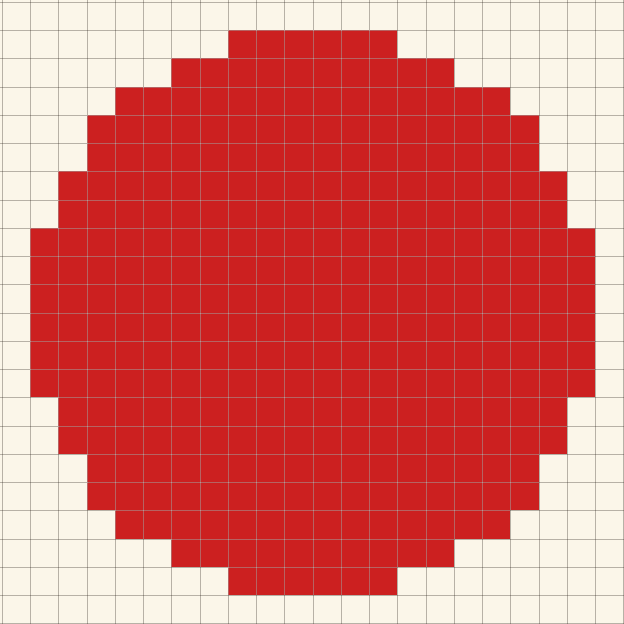
\includegraphics[width=\linewidth]{fig01_2d_d20_euclidean.png}
  \caption{\emph{Евклидов}}
\end{subfigure}\hfill
\begin{subfigure}[t]{0.31\linewidth}\centering
  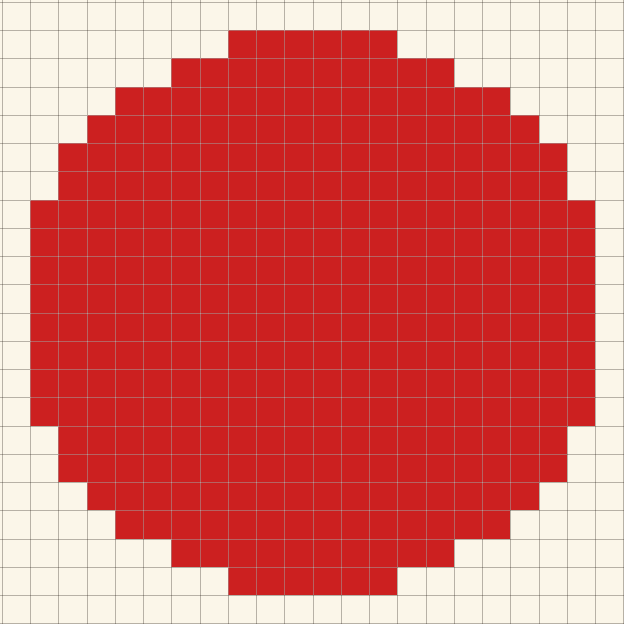
\includegraphics[width=\linewidth]{fig02_2d_d20_bresenham.png}
  \caption{\emph{Брезенхэма}}
\end{subfigure}\hfill
\begin{subfigure}[t]{0.31\linewidth}\centering
  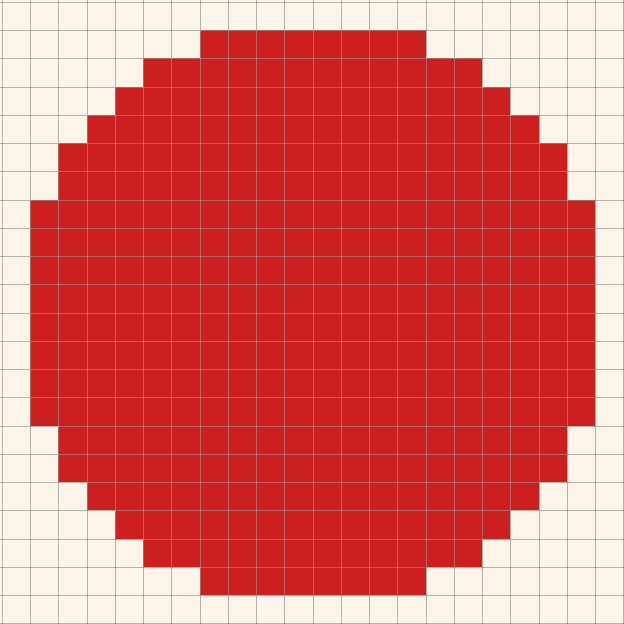
\includegraphics[width=\linewidth]{fig03_2d_d20_threshold.png}
  \caption{\emph{Пороговый}}
\end{subfigure}
\caption{Одна и та же окружность диаметра 20 в трёх алгоритмах. При больших диаметрах различия более тонкие, чем при малых.}
\label{fig:comp-d20}
\end{figure}


% =============================================================================
\subsection{Урок 3 --- ``От эллипса к эллипсоиду: третье измерение''}

\subsubsection*{Цель урока}
Обобщить уравнение эллипса на трёхмерный случай; ввести вокселы и дискретный объём; понять плоские сечения как линейные неравенства.

\begin{zadanie}[3.1 --- От 2D к 3D \quad\vrema{15 мин}]
Добавим третью координату $z$. Уравнение эллипса немедленно обобщается:

\begin{formula}
\centering
$\displaystyle \left(\dfrac{x}{r_x}\right)^{\!2} + \left(\dfrac{y}{r_y}\right)^{\!2} + \left(\dfrac{z}{r_z}\right)^{\!2} \;=\; 1$
\end{formula}

При $r_x = r_y = r_z = r$ получаем \acc{сферу} $x^2 + y^2 + z^2 = r^2$.

\textbf{Воксель.} Ячейка трёхмерной сетки называется \emph{воксель} (\emph{volume element}). Критерий принадлежности тот же, что и в двумерном случае:

\begin{formula}
\centering
$\displaystyle a_x^2 + a_y^2 + a_z^2 \leq 1,\quad a_\xi = \dfrac{\xi + \tfrac{1}{2} - c_\xi}{r_\xi}$
\end{formula}

\textbf{Демонстрация.} Переключить Pixel Round в режим 3D, попеременно показать \emph{Сферу} и \emph{Эллипсоид}, вращать мышью, обратить внимание на структуру вокселей и стили затенения (\emph{Classic, Smooth, Blocks}).
\end{zadanie}
\begin{figure}[H]
\centering
\begin{subfigure}[t]{0.42\linewidth}\centering
  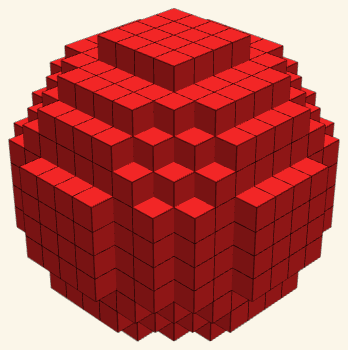
\includegraphics[width=\linewidth]{fig07_3d_sphere_d12.png}
  \caption{Сфера $D = 12$ ($r_x = r_y = r_z = 6$).}
\end{subfigure}\hfill
\begin{subfigure}[t]{0.42\linewidth}\centering
  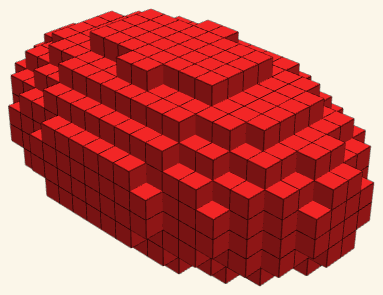
\includegraphics[width=\linewidth]{fig08_3d_ellipsoid.png}
  \caption{Эллипсоид $W = 20, H = 10, D = 12$.}
\end{subfigure}
\caption{Воксельная 3D-визуализация. Каждый куб — это воксель, координата центра которого проверяется по неявному уравнению.}
\label{fig:3d-shapes}
\end{figure}


\begin{zadanie}[3.2 --- Непрерывный и дискретный объём \quad\vrema{15 мин}]
Непрерывный объём эллипсоида --- классический результат интегрального исчисления:

\begin{formula}
\centering
$\displaystyle V \;=\; \dfrac{4}{3}\,\pi\, r_x\, r_y\, r_z$
\end{formula}

При $r_x = r_y = r_z = r$ получаем $V = \tfrac{4}{3}\pi r^3$. Эта формула регулярно появляется в задачах ЕГЭ профильного уровня (задание 13 или 14 в зависимости от года).

\textbf{Работа в парах:}
\begin{enumerate}[leftmargin=1.5em,itemsep=0.15em,topsep=0.3em,nosep]
  \item Вычислить непрерывный объём сферы диаметра 12 ($r = 6$): $V = \tfrac{4}{3}\pi \cdot 216 \approx 904{,}78$.
  \item В Pixel Round построить сферу $D = 12$ в режиме \emph{Заполненный}. Считать дискретный объём.
  \item Вычислить относительную погрешность.
\end{enumerate}

\textbf{Обсуждение:} отношение $V_{\text{дискр}}/V_{\text{непр}} \to 1$ при $D \to \infty$. При малых $D$ расхождение существенно --- и это \emph{математически правильно}: дискретизация действительно меняет подсчёт. Связь с классической \emph{проблемой Гаусса о точках в круге}.
\end{zadanie}

\begin{zadanie}[3.3 --- Сечения как линейные неравенства \quad\vrema{8 мин}]
Pixel Round позволяет рассекать твёрдое тело тремя плоскостями. Каждое сечение --- это \acc{линейное неравенство}, применённое к центру вокселя:

\begin{formula}
\centering
$\begin{array}{lcl}
\text{Ось X:} & x \geq \mathit{cut} & \Rightarrow \text{воксель отбрасывается} \\
\text{Ось Y:} & y \geq \mathit{cut} & \Rightarrow \text{воксель отбрасывается} \\
\text{Диагональ:} & x + y \geq \mathit{cut} & \Rightarrow \text{воксель отбрасывается}
\end{array}$
\end{formula}

\textbf{Демонстрация.} Рассечь сферу по оси Y на 50\%, затем по оси X на 50\%. Перейти к диагональному сечению при 50\% --- наблюдать срез под углом $45°$ в плоскости $xy$.

\textbf{Направляющий вопрос:} \emph{``Почему ползунок диагонального сечения изменяется от 0 до $D_x + D_y$, а не до $D_x$? Где в уравнении находится ответ?''}
\end{zadanie}
\begin{figure}[H]
\centering
\begin{subfigure}[t]{0.31\linewidth}\centering
  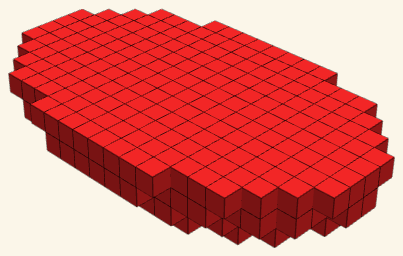
\includegraphics[width=\linewidth]{fig09_3d_cut_y50.png}
  \caption{Сечение Y на 50\% ($y \geq 5$ удалено)}
\end{subfigure}\hfill
\begin{subfigure}[t]{0.31\linewidth}\centering
  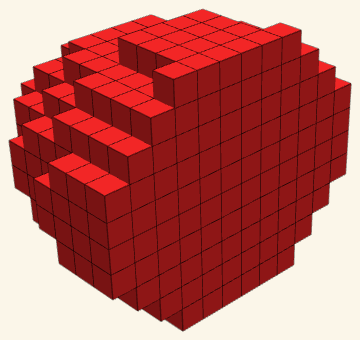
\includegraphics[width=\linewidth]{fig10_3d_cut_x50.png}
  \caption{Сечение X на 50\% ($x \geq 10$ удалено)}
\end{subfigure}\hfill
\begin{subfigure}[t]{0.31\linewidth}\centering
  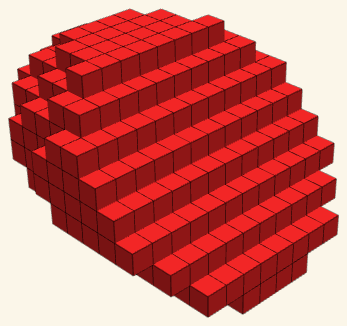
\includegraphics[width=\linewidth]{fig11_3d_cut_diag50.png}
  \caption{Диагональное сечение ($x + y \geq 15$ удалено)}
\end{subfigure}
\caption{Три плоских сечения одного и того же эллипсоида ($W = 20, H = 10, D = 12$), каждое сохраняет 50\% объёма. Обратите внимание на ступенчатый узор диагонального сечения.}
\label{fig:cortes}
\end{figure}


\begin{zadanie}[3.4 --- Культурно-исторический контекст \quad\vrema{7 мин}]
\emph{Связь с историей русского искусства начала XX века.}

Показать три изображения:
\begin{itemize}[leftmargin=1.3em,itemsep=0.1em,topsep=0.2em,nosep]
  \item Казимир Малевич --- ``Чёрный квадрат'' (1915) и его супрематические композиции с кругами и пересекающимися плоскостями.
  \item Александр Родченко --- графические композиции 1920-х годов с окружностями и геометрическими сечениями.
  \item Владимир Татлин --- проект ``Памятник III Интернационалу'' с двойной спиралью и сферическими формами.
\end{itemize}

\textbf{Обсуждение:} \emph{``Русские супрематисты сто лет назад уже мыслили окружность и квадрат как первоэлементы языка. Они работали с геометрическими формами как с строительными блоками визуального высказывания. Pixel Round, в каком-то смысле, делает то же самое --- но в среде, в которой ``строительные блоки'' жёстко определены математически. Что объединяет, а что разделяет эти два подхода?''}

Эта связь служит мостом к Изобразительному искусству и может развиваться в совместном проекте с учителем ИЗО или истории искусства.
\end{zadanie}

% =============================================================================
\subsection{Урок 4 --- ``Итоговый проект: авторская пиксельная графика с математической защитой''}

\subsubsection*{Цель урока}
Мобилизовать всё содержание серии в авторском продукте; оценить через защиту с обязательной математической аргументацией.

\begin{zadanie}[4.1 --- Введение в проект \quad\vrema{5 мин}]
\textbf{Задача:} \emph{``В парах или тройках вы создаёте изображение в стиле \emph{пиксельной графики} или \emph{воксельной графики}, объединяющее не менее трёх фигур, построенных в Pixel Round (окружности, эллипсы, сферы или эллипсоиды). Это может быть персонаж, иконка, животное, логотип --- выбор за вами. По окончании каждая группа представит работу, объясняя \acc{математически} принятые решения: почему этот алгоритм? почему такая пропорция? почему это сечение?''}

\textbf{Формирование групп:} заранее, по принципу разнородности.
\end{zadanie}

\begin{zadanie}[4.2 --- Производство \quad\vrema{30 мин}]
\textbf{Материал на группу:}
\begin{itemize}[leftmargin=1.3em,itemsep=0.15em,topsep=0.3em,nosep]
  \item Устройство с доступом к Pixel Round;
  \item Клетчатая бумага, карандаши, фломастеры для эскизов;
  \item Лист с тремя обязательными вопросами (Приложение~\ref{ap:zad}, задание~5).
\end{itemize}

\textbf{Внутренние этапы:}
\begin{enumerate}[leftmargin=1.5em,itemsep=0.15em,topsep=0.3em,nosep]
  \item \vrema{5 мин} обсуждение и эскиз на бумаге.
  \item \vrema{15 мин} работа в Pixel Round, экспорт частей в PNG.
  \item \vrema{5 мин} окончательная сборка (на клетчатой бумаге фломастерами или в цифровой презентации).
  \item \vrema{5 мин} письменное обоснование на листе с вопросами.
\end{enumerate}

\textbf{Сопровождение учителя:} обход групп с наводящими вопросами --- \emph{``почему вы выбрали этот алгоритм? как описать это сечение неравенством?''}
\end{zadanie}

\begin{zadanie}[4.3 --- Защита и итоговая рефлексия \quad\vrema{10 мин}]
Каждая группа располагает 2 минутами на презентацию работы и ответ хотя бы на один из трёх обязательных вопросов.

\textbf{Минимальные критерии:}
\begin{itemize}[leftmargin=1.3em,itemsep=0.1em,topsep=0.2em,nosep]
  \item Выделить хотя бы одну математическую фигуру;
  \item Назвать выбранный алгоритм и обосновать (хотя бы \emph{постфактум}) его пригодность;
  \item При наличии 3D-сечения --- записать его как неравенство.
\end{itemize}

\textbf{Итоговая рефлексия учителя (3 мин):} вернуться к основной идее серии --- \emph{``на дискретной сетке одна и та же непрерывная кривая допускает несколько представлений; выбор одного из них --- математическое решение''}. Объявить сроки сдачи карточки с заданиями.
\end{zadanie}

% =============================================================================
\section{Оценивание}

Оценивание построено в логике \acc{критериального формирующего оценивания}, отвечающего требованиям ФГОС СОО и поддерживающего подготовку к ЕГЭ. Используются три модуля.

\subsection{Диагностическое оценивание}
Урок~1, Задание~1.2. Учитель выявляет учащихся с пробелами в знании координатной плоскости, уравнения окружности, понятия площади.

\subsection{Формирующее оценивание}
Распределено по всем урокам: наблюдение за участием, качество индивидуальных ответов в Заданиях~1.4, 2.2, 2.5 и 3.2.

\subsection{Итоговое оценивание}
Два продукта:
\begin{enumerate}[leftmargin=1.5em,itemsep=0.2em,topsep=0.3em,nosep]
  \item \textbf{Карточка с заданиями} (Приложение~\ref{ap:zad}), 5 заданий, сдаётся по окончании Урока~4.
  \item \textbf{Итоговый проект} (Задание~4.2) с заполненным листом обоснования.
\end{enumerate}

\subsection{Критериальная рубрика}

\begin{center}
\small
\begin{tabularx}{\textwidth}{@{}p{0.21\textwidth}XX@{}}
\toprule
\textbf{Критерий} & \textbf{Освоен полностью (4--5 баллов)} & \textbf{Освоен частично (3 балла) / Не освоен (2)} \\
\midrule
\textbf{Математическое содержание} & Уверенно применяет уравнения эллипса и эллипсоида; различает три алгоритма и предсказывает их результат. & Применяет только уравнение окружности; путает алгоритмы. \\
\addlinespace[3pt]
\textbf{Владение программой} & Самостоятельно работает в Pixel Round в 2D и 3D; экспортирует; переключает режимы. & Требуется постоянная помощь; работает только в 2D. \\
\addlinespace[3pt]
\textbf{Аргументация} & Защищает решения проекта с использованием математической терминологии (алгоритм, воксель, сечение, неравенство). & Аргументирует только эстетически; терминология отсутствует. \\
\addlinespace[3pt]
\textbf{Сотрудничество} & Активно работает в паре или тройке; участвует в общей дискуссии. & Работает в одиночку; вклад минимален. \\
\bottomrule
\end{tabularx}
\end{center}

\subsection{Удельный вес в четвертной оценке}
\begin{itemize}[leftmargin=1.3em,itemsep=0.1em,topsep=0.2em,nosep]
  \item Карточка с заданиями: 40\%.
  \item Итоговый проект и защита: 50\%.
  \item Процессуальное наблюдение: 10\%.
\end{itemize}

% =============================================================================
\section{Межпредметные связи}

\subsection{С информатикой}
Алгоритм Брезенхэма входит в программу любого курса по основам алгоритмики. Урок~2.3 можно проводить совместно с учителем информатики, дополнив реализацией на Python. В рамках подготовки к ЕГЭ по информатике (задания 16 и 25) реализация целочисленного алгоритма --- отличная тренировка.

\subsection{С изобразительным искусством}
Пиксельная графика традиционно рассматривается в курсе ИЗО как форма цифрового искусства. Pixel Round даёт редкую возможность увидеть, как одна и та же фигура \emph{является} одновременно математическим объектом и эстетической композицией. Возможный совместный проект: выставка итоговых работ в школьном пространстве.

\subsection{С физикой}
Звуковой слой Pixel Round использует аддитивный синтез чистых синусоидальных волн. Выбранные частоты приближают ноты \acc{равномерно темперированного 12-тонового строя} (соседние полутоны различаются множителем $2^{1/12} \approx 1{,}0595$). Связь с темой \emph{Механические волны и звук}.

\subsection{С историей и обществознанием}
Алгоритм Брезенхэма опубликован в 1965 году --- в год запуска БЭСМ-6 в СССР, в эпоху космической гонки. Возможна параллель: \emph{параллельное развитие компьютерной графики в США и СССР, общие математические корни, разные институциональные траектории}. Эта тема может стать частью индивидуального проекта в 11 классе.

% =============================================================================
\section{Список литературы}

\begin{itemize}[leftmargin=1.3em,itemsep=0.2em,topsep=0.3em]
  \item Колмогоров А. Н. \emph{Современная математика и математика в современной школе}. Математика в школе, № 6, 1971.
  \item Лакатос И. \emph{Доказательства и опровержения. Как доказываются теоремы}. М.: Наука, 1967 [англ.~1976].
  \item Лобачевский Н. И. \emph{Полное собрание сочинений по геометрии}. М.: Гостехиздат, 1946.
  \item Минпросвещения России. \emph{Федеральный государственный образовательный стандарт среднего общего образования}. Приказ от 12.08.2022 № 732. М.: 2022.
  \item Понтрягин Л. С. \emph{Принцип максимума в оптимальном управлении}. М.: Наука, 1989.
  \item Пойа Д. \emph{Как решать задачу}. М.: Учпедгиз, 1959 [англ.~1945].
  \item Сосинский А. Б. \emph{Геометрия}. М.: МЦНМО, 2007.
  \item Тихомиров В. М. \emph{Рассказы о математиках}. М.: МЦНМО, 2007.
  \item Эльконин Д. Б., Давыдов В. В. \emph{Теория развивающего обучения}. М.: ИНТОР, 1996.
  \item Bresenham J. E. Algorithm for computer control of a digital plotter. \emph{IBM Systems Journal}, vol.~4, no.~1, pp.~25--30, 1965.
  \item Pitteway M. L. V. Algorithm for drawing ellipses or hyperbolae with a digital plotter. \emph{The Computer Journal}, vol.~10, no.~3, pp.~282--289, 1967.
  \item Pixel Round --- технический документ: \texttt{docs\_math/Pixel\_Round\_Math\_ru-RU.pdf}.
\end{itemize}

\newpage
% =============================================================================
% ПРИЛОЖЕНИЯ
% =============================================================================
\appendix
\renewcommand{\thesection}{\Alph{section}}
\setcounter{section}{0}

\section{Сценарий демонстрации Pixel Round}\label{ap:scenario}

Рекомендованная последовательность для демонстрации в Задании~1.3 и для самостоятельной подготовки учителя. Общая длительность: 15 минут.

\subsection{Запуск и режим 2D}
\begin{enumerate}[leftmargin=1.5em,itemsep=0.15em,topsep=0.3em]
  \item Открыть Pixel Round. Указать на верхнюю панель, центральную область рисования и панель управления.
  \item Подтвердить режим \acc{2D / Круг}.
  \item Установить ползунок \emph{Size} на значение 10.
  \item Активировать информационный значок. Зачитать: ``Диаметр 10, Радиус 5, Площадь \dots, Алгоритм Евклидов''.
  \item Переключить алгоритмы: \acc{Евклидов / Брезенхэм / Пороговый}. По 30 секунд на каждый.
\end{enumerate}

\subsection{Эллипс}
\begin{enumerate}[leftmargin=1.5em,itemsep=0.15em,topsep=0.3em]
  \item Сменить форму на \acc{Эллипс}. Появляются ползунки \emph{Ширина} и \emph{Высота}.
  \item Установить $W = 16$, $H = 8$.
  \item Вопрос: \emph{``Уравнение этой формы --- $(x/8)^2 + (y/4)^2 = 1$. Почему делим $x$ на 8, а $y$ --- на 4?''}
\end{enumerate}

\subsection{Режим 3D}
\begin{enumerate}[leftmargin=1.5em,itemsep=0.15em,topsep=0.3em]
  \item Переключиться на \acc{3D / Сфера}, $D = 12$.
  \item Вращать мышью.
  \item Активировать информационный значок: записать объём.
  \item Сменить форму на \acc{Эллипсоид}: $W = 20, H = 10, D = 10$.
  \item Продемонстрировать ползунок \emph{Cut} по оси $Y$, 50\%.
  \item Перейти на диагональную ось. Обсудить диагональное сечение.
\end{enumerate}

\subsection{Экспорт}
\begin{enumerate}[leftmargin=1.5em,itemsep=0.15em,topsep=0.3em]
  \item Кнопка скачивания в углу области рисования.
  \item Сохранить PNG.
  \item Отметить высокое разрешение --- пригодное для печати и проекции.
\end{enumerate}

% =============================================================================
\newpage
\section{Карточка с заданиями}\label{ap:zad}

\textbf{Указания.} Работа индивидуальная. Допустимо сверяться с Pixel Round, \emph{но математическое обоснование обязательно}. Сдать в письменном или печатном виде.

\subsection*{Задание 1 --- Уравнение окружности}
\textbf{Условие.} Окружность с центром в начале координат и радиусом $r = 7$. Для каждой точки определить, находится ли она \emph{внутри}, \emph{вне} или \emph{на} окружности. Обосновать.
\begin{enumerate}[label=\alph*),leftmargin=1.5em,itemsep=0.1em,topsep=0.2em,nosep]
  \item $(3, 4)$ \hfill \emph{ответ:} внутри ($25 < 49$).
  \item $(5, 5)$ \hfill \emph{ответ:} вне ($50 > 49$).
  \item $(0, 7)$ \hfill \emph{ответ:} на.
  \item $(-7, 0)$ \hfill \emph{ответ:} на.
\end{enumerate}

\subsection*{Задание 2 --- Евклидов критерий}
\textbf{Условие.} Окружность с центром $(5, 5)$ и радиусом $5$. Применить евклидов критерий к ячейке $(1, 3)$: закрашивается ли она?

\emph{Ответ:} центр ячейки $(1{,}5,\, 3{,}5)$. Расстояние: $\sqrt{14{,}5} \approx 3{,}81 < 5$. Ячейка \acc{закрашивается}.

\subsection*{Задание 3 --- Дискретная и непрерывная площадь}
\textbf{Условие.} В Pixel Round построить окружность диаметром 20 в евклидовом режиме. Записать дискретную площадь. Вычислить непрерывную $\pi r^2$. Найти относительную погрешность. Повторить для порогового алгоритма. Сравнить.

\emph{Ответ:} $S_{\text{непр}} = 100\pi \approx 314{,}16$. Евклидов: погрешность < 2\%. Пороговый: завышение на 5--8\%.

\subsection*{Задание 4 --- Объём эллипсоида и сечение}
\textbf{Условие.} Полуоси эллипсоида $r_x = 4$, $r_y = 6$, $r_z = 3$.
\begin{enumerate}[label=\alph*),leftmargin=1.5em,itemsep=0.1em,topsep=0.2em,nosep]
  \item Найти непрерывный объём.
  \item После сечения по оси $Y$, сохраняющего 50\% высоты, найти остаточный объём.
  \item Описать сечение неравенством на координате $y$.
\end{enumerate}

\emph{Ответ:}
(а) $V = 96\pi \approx 301{,}59$.
(б) По симметрии $\approx 150{,}80$.
(в) $y < \mathit{cut}$, $\mathit{cut} = 6$.

\subsection*{Задание 5 --- Лист обоснования итогового проекта}
\textbf{Условие.} После создания работы в группе ответить:
\begin{enumerate}[label=(\arabic*),leftmargin=1.7em,itemsep=0.15em,topsep=0.2em,nosep]
  \item Перечислить использованные геометрические фигуры с их параметрами.
  \item Для главной фигуры: какой алгоритм выбран? Почему? Какой визуальный эффект он даёт, недоступный другим двум?
  \item Использовалось ли 3D-сечение? Если да, описать \emph{одно} из них неравенством.
\end{enumerate}

% =============================================================================
\newpage
\section{Адаптация для школ с ограниченной материальной базой}\label{ap:adapt}

Эта адаптация позволяет провести всю серию \emph{полностью на бумаге} в случаях, когда доступ к компьютерам не обеспечен для всей группы. Содержательное ядро остаётся неизменным; меняется только материальная основа.

\subsection{Замены по урокам}

\begin{center}
\small
\begin{tabularx}{\textwidth}{@{}p{0.16\textwidth}p{0.36\textwidth}X@{}}
\toprule
\textbf{Урок} & \textbf{Оригинальное задание} & \textbf{Аналоговая замена} \\
\midrule
1 & Демонстрация Pixel Round (1.3) & Учитель чертит три версии окружности $D = 10$ на заранее размеченной клетчатой области большого формата (плакат A2 или больше). \\
\addlinespace[3pt]
2 & Программное сравнение (2.5) & Раздать заранее распечатанные карточки с тремя окружностями $D = 16$; ручной подсчёт ячеек. \\
\addlinespace[3pt]
3 & Построение 3D-сферы (3.1, 3.2) & Раздать листы со \emph{срезами} сферы ($z = 0, 1, 2, \ldots$) на клетчатой бумаге. Мысленное сложение в трёхмерное тело. \\
\addlinespace[3pt]
4 & Производство в Pixel Round (4.2) & Создание \emph{исключительно} на клетчатой бумаге цветными карандашами. Защита (4.3) проходит без изменений. \\
\bottomrule
\end{tabularx}
\end{center}

\subsection{Комплект подготовки (одноразовый)}
\begin{itemize}[leftmargin=1.3em,itemsep=0.1em,topsep=0.2em,nosep]
  \item Один лист A3 с клетчатой сеткой $30 \times 30$, расчерченный учителем и прикреплённый к доске или стене.
  \item На каждого учащегося набор из 4 листов A4 в клетку (5\,мм).
  \item Один лист с тремя сравнительными окружностями $D = 16$, заранее построенный учителем в Pixel Round, экспортированный и распечатанный в школьной канцелярии.
\end{itemize}

\subsection{Региональная специфика}

Россия отличается значительной географической и социально-экономической неоднородностью. Серия уроков сознательно построена так, чтобы быть применимой:

\begin{itemize}[leftmargin=1.3em,itemsep=0.15em,topsep=0.3em]
  \item в специализированных физико-математических школах (СУНЦ МГУ, Президентский физико-математический лицей №\,239, Лицей №\,131 Казани, ФМЛ №\,2 Кирова): см.~расширенные задания в §\ref{sec:diff}.
  \item в массовой городской школе: основной маршрут, описанный в технологической карте.
  \item в сельских и удалённых школах: предложенная аналоговая адаптация, дополненная при возможности кратким сеансом работы с одним демонстрационным ноутбуком учителя.
\end{itemize}

% =============================================================================
\newpage
\section{Терминологический словарь для учителя}\label{ap:glos}

\begin{itemize}[leftmargin=1.4em,itemsep=0.3em,topsep=0.3em]
  \item \acc{Алгоритм} --- конечная, чётко определённая последовательность инструкций для решения задачи. Три алгоритма Pixel Round --- разные процедуры для одной и той же задачи.
  \item \acc{Алгоритм Брезенхэма} --- алгоритм, опубликованный в 1965 году Джеком Брезенхэмом (IBM) для отрезков прямой, позже распространённый на окружности и эллипсы (Питуэй, Каппель). Отличительная черта --- целочисленная арифметика.
  \item \acc{Canvas (холст)} --- HTML-элемент, предоставляющий область двумерного или трёхмерного рисования в браузере.
  \item \acc{Неявное уравнение} --- уравнение вида $F(x, y) = 0$, в котором кривая определяется как множество нулей функции. Для эллипса: $(x/r_x)^2 + (y/r_y)^2 - 1 = 0$.
  \item \acc{Пиксель} --- сокращение от \emph{picture element}. Минимальная единица цифрового изображения; в сетке занимает ячейку $1 \times 1$.
  \item \acc{PWA --- Progressive Web App} --- веб-приложение, устанавливаемое на устройство и работающее в офлайн-режиме. Pixel Round является PWA.
  \item \acc{Растеризация} --- преобразование непрерывного геометрического описания в матрицу пикселей (2D) или вокселей (3D).
  \item \acc{Полуось} --- в эллипсе с центром $C$: расстояние от $C$ до вершины эллипса вдоль соответствующей оси. Окружность --- частный случай $r_x = r_y$.
  \item \acc{Равномерно темперированный 12-тоновый строй} --- деление октавы на 12 равных полутонов. Отношение частот двух смежных полутонов: $\sqrt[12]{2} \approx 1{,}0595$. Основа западной и большей части русской классической музыки.
  \item \acc{Воксель} --- сокращение от \emph{volume element}. Трёхмерное обобщение пикселя: кубическая ячейка $1 \times 1 \times 1$.
  \item \acc{WebGL} --- библиотека для трёхмерной графики в браузере. Pixel Round использует её через \emph{three.js}.
\end{itemize}

\vspace{2em}
\begin{center}
\color{muted}\small\sffamily
--- конец технологической карты ---
\end{center}

\end{document}
